\documentclass{article}

\usepackage[dblblindworkshop]{neurips_2026}
\workshoptitle{New In ML at NeurIPS 2026}

\usepackage[utf8]{inputenc}
\usepackage[T1]{fontenc}
\usepackage{hyperref}
\usepackage{url}
\usepackage{booktabs}
\usepackage{amsmath}
\usepackage{amsfonts}
\usepackage{amssymb}
\usepackage{graphicx}
\usepackage{microtype}
\usepackage{xcolor}
\usepackage{multirow}
\usepackage{tabularx}
\usepackage{tikz}
\usetikzlibrary{arrows.meta,backgrounds,fit,positioning}
\hypersetup{hidelinks}

\title{SpeechGR: Exploring End-to-End Textless Speech Generative Retrieval}

% The review style replaces this block with anonymous author information.
\author{Anonymous Author(s)}

\begin{document}

\maketitle

\begin{abstract}
In the formulation studied here, generative retrieval (GR) retrieves by
generating corpus identifiers rather than ranking stored document embeddings.
Among the systems considered here, IRGen provides the closest structural
analogue: a raw image generates a valid identifier for a relevant database
image. GENIUS also accepts visual query content, but pairs each query with a
natural-language task instruction and uses CLIP-based, contrastively aligned
encoders. We study whether the same retrieval paradigm can operate over speech.
In SLUE-SQA-5, relevance is directional: a spoken question is linked to
an answer-containing spoken passage using text-retrieval and QA criteria rather
than acoustic distance. SpeechGR quantizes questions
and passages into discrete HuBERT units, adapts a Flan-T5 encoder--decoder, and
generates valid passage identifiers with trie-constrained decoding rather than
ANN search. It uses neither an intermediate ASR transcript nor a textual query
instruction. On a 15,883-passage SLUE-SQA-5 collection, SpeechGR reaches
5.81\% Hit@1 and 18.452\% Hit@20. Speech-unit span-corruption pretraining gives
the strongest positive pattern, whereas the tested BPE, ranking-loss, and
Q-Former variants score below their reported references. These results
establish feasibility for spoken-question DocID generation. Because the
benchmark is text-derived and the model remains text-pretrained, the experiment
does not isolate semantic reasoning from lexical correspondence.
\end{abstract}

\newcommand{\PaperIntroduction}{%
\section{Introduction}
\label{sec:introduction}

Generative retrieval (GR) learns to produce a document identifier (DocID) from
a query rather than searching stored document embeddings
\citep{Tay2022TransformerMA,Li2024FromMT}. Among the systems considered here,
IRGen provides the closest structural precedent for a non-text query: a query
image is encoded and a valid database-image identifier is generated
autoregressively
\citep{Zhang2024IRGen}. Its task is same-modality image retrieval, with
relevance defined by shared dataset class labels. GENIUS broadens GR to
text, image, and image--text query content, but each query is conditioned on a
natural-language task instruction and embedded through CLIP-based
vision--language alignment \citep{Kim2025GENIUSAG}. These results establish
non-text-query GR in vision, but not direct spoken-query identifier generation.

The QA retrieval setting introduces a different relevance relation. A spoken
question is paired with a passage because the passage contains the answer, not
because the two recordings are acoustically similar. They may differ in
speaker, duration, wording, and recording conditions. The resulting mapping is
asymmetric: question \(\rightarrow\) answer-containing passage. Spoken retrieval
usually handles this abstraction through ASR followed by text retrieval, or
through dense representations searched in an external vector index
\citep{Wang2023AVATARRV,Lin2024SpeechDPRES}. The former inherits transcription
errors and imposes a text interface; the latter retains embedding search. We
therefore ask: \emph{can a generative retriever map a spoken question directly
to an answer-containing spoken passage when relevance is not defined by acoustic
similarity and no intermediate transcript is available?}

Discrete speech units make this question compatible with sequence models by
turning audio into token sequences without transcribing it
\citep{Hsu2021HuBERTSS,lakhotia-etal-2021-generative,lin22c_interspeech}. The
retriever generates a DocID without querying an external document-embedding
index or performing ANN search. A prefix trie restricts decoding to valid
DocIDs; it is an output constraint rather than a dense retrieval index.

We study \textbf{SpeechGR}, which quantizes spoken questions and passages into
discrete acoustic units and trains a Flan-T5 encoder--decoder to generate the
identifier of an answer-containing passage. The model learns jointly from
passage-to-DocID indexing examples and spoken-query-to-DocID retrieval examples,
and its model inputs consume neither query/passage transcripts nor a textual
query instruction during SpeechGR training or inference. Flan-T5 nevertheless
contributes text pretraining. On the English SLUE-SQA-5 benchmark
\citep{Shon2022SLUEPA},
SpeechGR obtains 5.81 Hit@1 and 18.452 Hit@20 over the 15,883 passages in the
current data export. Speech-unit pretraining provides the strongest positive
experimental pattern, while BPE compression, pairwise ranking loss, and a
windowed Q-Former do not improve their reported references. Gold-text and prior
speech retrievers are reported only as contextual evidence because their
inputs, supervision, mechanisms, or candidate pools differ.

This work makes three contributions:
\begin{itemize}
    \item We study spoken-question generative passage retrieval, in which a
    spoken question generates the identifier of its linked answer-containing
    passage; relevance labels are not based on acoustic similarity.
    \item We develop SpeechGR, which maps discrete speech units to valid
    passage identifiers without consuming task transcripts or textual query
    instructions and retrieves without dense ANN search.
    \item We establish feasibility on a 15,883-passage SLUE-SQA-5 collection
    and report scoped evidence on acoustic units, speech pretraining,
    identifier design, and compression and ranking variants that did not help.
\end{itemize}
}

\newcommand{\PaperRelatedWork}{%
\section{Related Work}
\label{sec:related-work}

\paragraph{Generative retrieval.}
In the standard formulation used here, GR replaces nearest-neighbor search
with autoregressive DocID generation. DSI established the parameterized-index
formulation \citep{Tay2022TransformerMA}; later work studies identifier design,
query generation, and retrieval training
\citep{Zhuang2022BridgingTG,Li2024FromMT,Kuo2024ASO}. Valid-identifier tries
commonly constrain decoding \citep{DeCao2020AutoregressiveER}. Cross-modal GR
generates identifiers for image, audio, and video targets from text queries
\citep{li-etal-2024-generative,fang-etal-2025-cart,
fang25c_interspeech}. IRGen instead maps a raw image to codes for neighboring
images, learns retrieval-specific visual identifiers, and evaluates up to
million-scale collections \citep{Zhang2024IRGen}. It is structurally analogous
to SpeechGR, but evaluates same-modality image retrieval using shared class
labels.
GENIUS accepts visual query content, yet also supplies a textual task
instruction and uses a CLIP-aligned multimodal encoder
\citep{Kim2025GENIUSAG}. SpeechGR instead studies speech-only query content and
an asymmetric question-to-passage relation; its task inputs include neither a
transcript nor a natural-language retrieval instruction.

\paragraph{Spoken retrieval.}
ASR-based pipelines expose downstream retrieval to transcription errors;
AVATAR explicitly studies robustness to such noise
\citep{Wang2023AVATARRV}. SpeechDPR instead learns speech representations for a
dense retriever and distills semantics from an unsupervised ASR model and a
text retriever \citep{Baevski2021UnsupervisedSR,Lin2024SpeechDPRES}. SpeechGR
complements these systems with an ASR-free mapping from a spoken question to an
answer-containing passage DocID rather than using external dense passage
search. Recent dense retrievers report substantially higher SLUE-SQA-5 recall
while importing
strong text-side structure. CLSR optimizes ASR objectives and maps speech to
text-like representations consumed by a frozen BGE encoder
\citep{hu2026clsr}. WavRAG adapts an audio-language model on roughly 1.5
million mixed-modality retrieval examples, including text retrieval corpora
and TTS-derived speech \citep{chen-etal-2025-wavrag}. Their reported candidate
pools are not specified well enough to match SpeechGR's evaluation, but their
training signals clarify that transcription-free inference does not imply
text-independent retrieval learning.

\paragraph{Broader spoken-query benchmarks.}
The Massive Sound Embedding Benchmark (MSEB) introduces Simple Voice Questions
(SVQ), with more than 170k short spoken queries across 26 locales, 17
languages, and four recording conditions. It covers document, passage, and span
retrieval in both in-language and cross-language settings
\citep{Heigold2025MSEB}. Its recordings are readings of XTREME-UP text prompts
and query a textual Wikipedia index. SVQ therefore broadens multilingual and
acoustic-condition coverage, but remains speech-to-text retrieval rather than
speech-to-speech generative DocID retrieval.

\paragraph{A text-derived speech benchmark.}
SLUE-SQA-5 uses natural recordings, but derives questions from five text QA
datasets and pairs passages through transcript-side matching and retrieval
\citep{Shon2022SLUEPA}. Models also rely predominantly on lexical information
when lexical and prosodic cues coexist \citep{chi-etal-2025-role}. We therefore
treat it as a natural-speech realization of a lexically defined retrieval
problem, not a test that isolates speech-specific semantics.

\paragraph{Discrete speech units.}
Self-supervised speech encoders such as HuBERT can be clustered into discrete
units \citep{Hsu2021HuBERTSS}. Such units support generative spoken-language
modeling and downstream spoken understanding without requiring transcripts as
model inputs \citep{lakhotia-etal-2021-generative,lin22c_interspeech,
Shon2024DiscreteSLUAL}. We use them as the input vocabulary of a generative
retriever and examine how layer choice, codebook size, and sequence compression
affect retrieval.
}

\newcommand{\PaperLimitations}{%
\section{Limitations}
\label{sec:limitations}

The evidence is limited to English SLUE-SQA-5 and its linked Spoken Wikipedia
collection, so it does not establish multilingual performance, effectiveness
for unwritten languages, or scaling behavior on substantially larger
collections. The results also do not establish semantic reasoning. SLUE-SQA-5
is derived from text QA data and
transcript-based passage selection, so lexical correspondence may account for
part of the observed retrieval. Controlled paraphrase, low-overlap, and
acoustic-distractor evaluations would be needed to separate semantic mapping
from lexical pattern matching. SpeechGR is task-transcript-free rather than
text-independent: Flan-T5 is text-pretrained and the identifiers are
metadata-derived. IRGen and GENIUS are structural, not numerical, comparators:
class-based image retrieval, instruction-conditioned multimodal search, and
question-to-passage retrieval use different relevance labels and scales. The comparison with
SpeechDPR is neither supervision- nor candidate-pool-matched: SpeechGR uses
15,883 paired passages, whereas SpeechDPR reports retrieval over roughly 39k
Spoken Wikipedia segments. The CLSR and WavRAG candidate pools are
under-specified, and all of their values are imported rather than reproduced.
The gold-text BM25 reference uses one fixed tokenizer and parameter setting and
is not a sparse-retrieval sensitivity study.
The thesis does not report repeated runs, confidence intervals, or significance
tests.
The experimental record also does not preserve the per-ablation split and shared
pretraining setting, input-truncation policy, indexing/retrieval sampling
ratio, optimization hyperparameters, or completed-beam scoring needed for
exact reproduction; it is internally inconsistent about whether the
\(k\)-means codebook used 100 or 960 hours of LibriSpeech. Small differences
should therefore be interpreted cautiously. Finally, the experiments do not
evaluate corpus updates or retraining cost when passages change.
}

\newcommand{\PaperConclusion}{%
\section{Conclusion}
\label{sec:conclusion}

SpeechGR transfers the identifier-generation structure used in visual
retrieval to an asymmetric spoken task: a spoken question generates the DocID
of an answer-containing spoken passage. It uses no task transcript, textual query
instruction, or external document-embedding index. Its 5.81 Hit@1 and 18.452
Hit@20 on 15,883 SLUE-SQA-5 passages establish feasibility rather than parity
with text-guided retrieval. Speech-unit pretraining gives the strongest
positive pattern; the tested BPE, ranking-loss, and Q-Former variants do not.
Because the benchmark is text-derived, these results show learnable
question-to-passage associations but do not isolate semantic reasoning from
lexical matching. That distinction is the central challenge for future spoken
generative retrieval.
}


\PaperIntroduction
\PaperRelatedWork

\section{SpeechGR}
\label{sec:method}

\paragraph{Task formulation.}
Let \(\mathcal{C}=\{(p_i,y_i)\}_{i=1}^{N}\) be a corpus of spoken
passages, where \(p_i\) is an audio segment and \(y_i\) is its unique
document identifier (DocID). Let
\(\mathcal{Q}=\{(q_j,t(j))\}_{j=1}^{M}\) map each spoken query \(q_j\) to its
gold passage \(p_{t(j)}\). SpeechGR learns an encoder--decoder model
\(P_\theta(y\mid \mathbf{u}(q))\) and ranks passages by the probability of their
identifiers. Both queries and passages are represented as acoustic tokens.
The SLUE-SQA-5 relevance relation differs from IRGen's same-modality image
task: the gold passage is labelled because its transcript contains information
that answers the question, not because the query and passage recordings are
acoustically similar. SpeechGR is therefore trained to predict a directed
question-to-passage association rather than an acoustically similar recording.
Because SLUE-SQA-5 is text-derived, the experiment cannot determine how much
of this association reflects semantic reasoning rather than lexical
correspondence. Unlike IRGen's learned visual codes, SpeechGR generates
corpus-provided metadata DocIDs; their question-to-passage associations are
learned through the joint indexing and retrieval paths below.

We use \emph{end-to-end} for the ASR-free retrieval path from speech units to
DocIDs, not for joint optimization of the frozen HuBERT--\(k\)-means frontend
with the retriever. We use \emph{textless} for task inputs: SpeechGR's
acoustic-unit adaptation, retrieval fine-tuning, and inference do not consume
query or passage transcripts or a natural-language retrieval instruction.
Flan-T5 is nevertheless text-pretrained, and the DocIDs are metadata-derived
strings. We call this setup
\emph{index-free} in the standard generative-retrieval sense: inference does
not store passage embeddings or perform approximate nearest-neighbour (ANN)
search.  The valid-DocID trie used during decoding is an output constraint,
not an embedding index or similarity-search structure.

\begin{figure}[t]
    \centering
    \resizebox{\linewidth}{!}{%
    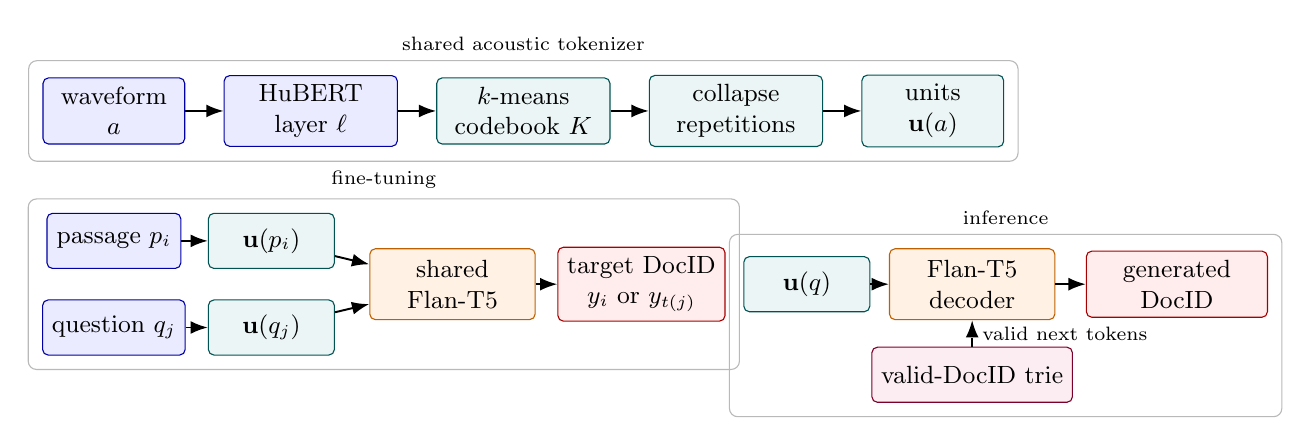
\begin{tikzpicture}[
        font=\small,
        >=Latex,
        flow/.style={-{Latex[length=2.2mm]}, line width=0.7pt},
        audio/.style={draw=blue!65!black, fill=blue!8, rounded corners=2pt,
            minimum height=7mm, align=center},
        units/.style={draw=teal!65!black, fill=teal!8, rounded corners=2pt,
            minimum height=7mm, align=center},
        model/.style={draw=orange!75!black, fill=orange!10, rounded corners=2pt,
            minimum height=9mm, align=center},
        output/.style={draw=red!65!black, fill=red!7, rounded corners=2pt,
            minimum height=7mm, align=center},
        constraint/.style={draw=purple!65!black, fill=purple!7,
            rounded corners=2pt, minimum height=7mm, align=center}
    ]
        % Shared acoustic tokenizer.
        \node[audio, minimum width=18mm] (wave) at (0,3.4) {waveform\\\(a\)};
        \node[audio, minimum width=22mm] (hubert) at (2.5,3.4) {HuBERT\\layer \(\ell\)};
        \node[units, minimum width=22mm] (kmeans) at (5.2,3.4) {\(k\)-means\\codebook \(K\)};
        \node[units, minimum width=22mm] (dedup) at (7.9,3.4) {collapse\\repetitions};
        \node[units, minimum width=18mm] (useq) at (10.4,3.4) {units\\\(\mathbf{u}(a)\)};
        \draw[flow] (wave) -- (hubert);
        \draw[flow] (hubert) -- (kmeans);
        \draw[flow] (kmeans) -- (dedup);
        \draw[flow] (dedup) -- (useq);

        % Fine-tuning: indexing and retrieval examples share parameters.
        \node[audio, minimum width=17mm] (passage) at (0,1.75)
            {passage \(p_i\)};
        \node[units, minimum width=16mm] (pu) at (2.0,1.75)
            {\(\mathbf{u}(p_i)\)};
        \node[audio, minimum width=17mm] (query) at (0,0.65)
            {question \(q_j\)};
        \node[units, minimum width=16mm] (qu) at (2.0,0.65)
            {\(\mathbf{u}(q_j)\)};
        \node[model, minimum width=21mm] (t5) at (4.3,1.2)
            {shared\\Flan-T5};
        \node[output, minimum width=20mm] (target) at (6.7,1.2)
            {target DocID\\\(y_i\) or \(y_{t(j)}\)};
        \draw[flow] (passage) -- (pu);
        \draw[flow] (query) -- (qu);
        \draw[flow] (pu) -- (t5);
        \draw[flow] (qu) -- (t5);
        \draw[flow] (t5) -- (target);

        % Inference: the trie constrains decoder scores, not a gold target.
        \node[units, minimum width=16mm] (infq) at (8.8,1.2)
            {\(\mathbf{u}(q)\)};
        \node[model, minimum width=21mm] (decoder) at (10.9,1.2)
            {Flan-T5\\decoder};
        \node[output, minimum width=23mm] (generated) at (13.5,1.2)
            {generated\\DocID};
        \node[constraint, minimum width=22mm] (trie) at (10.9,0.05)
            {valid-DocID trie};
        \draw[flow] (infq) -- (decoder);
        \draw[flow] (decoder) -- (generated);
        \draw[flow, dashed] (trie) -- node[right, font=\scriptsize]
            {valid next tokens} (decoder);

        \begin{scope}[on background layer]
            \node[draw=gray!55, rounded corners=3pt, inner sep=5pt,
                fit=(wave)(hubert)(kmeans)(dedup)(useq),
                label={[font=\scriptsize]above:shared acoustic tokenizer}] {};
            \node[draw=gray!55, rounded corners=3pt, inner sep=5pt,
                fit=(passage)(query)(pu)(qu)(t5)(target),
                label={[font=\scriptsize]above:fine-tuning}] {};
            \node[draw=gray!55, rounded corners=3pt, inner sep=5pt,
                fit=(infq)(decoder)(generated)(trie),
                label={[font=\scriptsize]above:inference}] {};
        \end{scope}
    \end{tikzpicture}%
    }
    \caption{\textbf{SpeechGR overview.} A shared HuBERT--\(k\)-means
    preprocessor maps passages and queries to deduplicated acoustic units.
    Fine-tuning combines passage-to-DocID indexing examples and
    spoken-question-to-answer-passage-DocID retrieval examples. At inference, a trie masks
    invalid next-token continuations during beam search; it stores valid output
    prefixes, not document embeddings.}
    \label{fig:speechgr}
\end{figure}


\subsection{Discrete speech units}
\label{sec:units}

Given an audio waveform \(a\), a pretrained HuBERT encoder
\citep{Hsu2021HuBERTSS} produces frame representations
\(\mathbf{z}_{1:T}\), with \(\mathbf{z}_t\in\mathbb{R}^{d}\).  We quantize
each frame using a \(k\)-means codebook
\(\mathcal{K}=\{\mathbf{c}_1,\ldots,\mathbf{c}_K\}\):
\begin{equation}
    u_t=\arg\min_{j\in\{1,\ldots,K\}}
    \lVert\mathbf{z}_t-\mathbf{c}_j\rVert_2^2 .
    \label{eq:quantization}
\end{equation}
This yields the discrete sequence
\(\mathbf{u}(a)=(u_1,\ldots,u_T)\).  Consecutive repetitions are collapsed,
so a run \(u_t=\cdots=u_{t+r}\) contributes one token.  This removes much of
the frame-rate redundancy without requiring a transcript.  We also test byte
pair encoding (BPE), following prior acoustic-unit work
\citep{Wang2024ACS}, as an optional second compression stage that merges
frequent adjacent units.  BPE is an ablation rather than part of the final
SpeechGR pipeline. Section~\ref{sec:analysis} reports the two same-\(K\)
comparisons available in the experiment record. The final reported
configuration uses HuBERT-large layer~22, \(K=500\), and deduplication without
BPE.

\subsection{Identifiers and model adaptation}
\label{sec:identifier-model}

The main identifier design uses the corpus-provided DocIDs.  These are short
character strings that encode corpus metadata, such as an article prefix and
sentence offset, and are tokenized into output sequences by the model
tokenizer.  We additionally study unstructured atomic identifiers, assigning
one distinct identifier to each passage, as an ablation motivated by
non-text generative retrieval \citep{li-etal-2024-generative}.  The main
system retains the corpus-provided string identifiers because they give the
better Hit@20 in our experiments.

SpeechGR uses Flan-T5-base \citep{10.5555/3722577.3722647} as its
encoder--decoder backbone.  To accept the acoustic sequence
\(\mathbf{u}(a)\), we expand its vocabulary with one entry per discrete unit.
Each added embedding is initialized by copying the vector of an unused token
in the original text vocabulary and remains trainable thereafter.  The
pretrained text vocabulary is retained for sentinel symbols and DocID
generation.

\subsection{Speech-unit pretraining}
\label{sec:speech-pretraining}

Before retrieval training, we adapt the expanded model to acoustic-token
sequences using the T5 span-corruption objective
\citep{Raffel2019ExploringTL}.  On a 6,000-hour subset of LibriLight, 15\% of
the units are grouped into contiguous spans and replaced by distinct sentinel
tokens; the decoder reconstructs the removed spans in order.  The final model
uses ten epochs of this pretraining.  Importantly, this stage adapts the
expanded encoder--decoder to discrete speech units; it does
\emph{not} teach the model the target Spoken Wikipedia passage-to-DocID
mapping.  Those corpus associations are learned only in the next stage.

\subsection{Joint indexing and retrieval training}
\label{sec:training}

Retrieval training combines two kinds of sequence-to-sequence examples,
following the two roles of a generative retriever
\citep{Tay2022TransformerMA}.  The \emph{indexing path} maps each spoken
passage to its own identifier,
\[
    \mathbf{u}(p_i)\longrightarrow y_i ,
\]
thereby associating corpus content with a DocID in the model parameters.  The
\emph{retrieval path} maps a spoken query to the identifier of its labelled
passage,
\[
    \mathbf{u}(q_j)\longrightarrow y_{t(j)} .
\]
Both paths use the same discrete-unit preprocessing and update the shared
Flan-T5 encoder--decoder on longer passage inputs and shorter query inputs.
For either training pair
\((\mathbf{x},\mathbf{y})\), where
\(\mathbf{y}=(y_1,\ldots,y_L)\), SpeechGR minimizes token-level
cross-entropy:
\begin{equation}
    \mathcal{L}_{\mathrm{CE}}(\mathbf{x},\mathbf{y})
    =-\sum_{\ell=1}^{L}
    \log P_\theta(y_\ell\mid y_{<\ell},\mathbf{x}) .
    \label{eq:ce}
\end{equation}
The paper's ranking-loss and windowed Q-Former variants are evaluated
separately in Section~\ref{sec:analysis}; neither is used in the final method.

\subsection{Constrained retrieval}
\label{sec:decoding}

At inference, SpeechGR converts only the spoken query to discrete units and
generates a DocID autoregressively.  We build a trie from the tokenized DocIDs
of all passages in \(\mathcal{C}\).  At every decoding step, tokens that do not
extend the current prefix along a trie edge are masked; completed hypotheses
therefore correspond to valid corpus passages.  Beam search retains the 20
highest-scoring prefixes, and completed beams give the ranked retrieval list.
This constraint prevents invalid identifiers but does not compare the query
against stored passage vectors, preserving the index-free GR formulation
defined above.

\section{Experiments}
\label{sec:experiments}

\subsection{Experimental setup}

\paragraph{Data and evaluation.}
We use the speech-to-speech retrieval setting introduced by
SpeechDPR~\citep{Lin2024SpeechDPRES}. Spoken questions come from SLUE-SQA-5
and candidate passages are the linked Spoken Wikipedia recordings
\citep{Shon2022SLUEPA}. The official train, validation, test, and
verified-test splits contain 46,186, 1,939, 2,382, and 408 questions. The
current SpeechGR metadata export contains 15,883 unique linked passages and
100\% coverage of the test gold identifiers. Each query has one gold passage.
We report Hit@1 and Hit@20, the percentage of queries for which that passage
appears in the first one or twenty generated identifiers. The headline result
uses the reported test split. The ablations are presented as development-stage
experiments, but the evaluation split and shared pretraining setting are not
recorded for every row. We therefore interpret them as comparisons among the
stated configurations rather than repeated-run or test-set effects.

The audio is natural, but the retrieval semantics are text-derived. Questions
come from five text QA datasets and were read by crowd workers; candidate
passages were paired using transcripts, answer-string matching, BM25,
sentence-level text retrieval, and text QA models
\citep{Shon2022SLUEPA}. Thus, relevance is answer-based rather than acoustic,
but the construction may reward lexical overlap. This makes clean-text
retrieval an important reference while preventing strong claims about
speech-specific semantics or compositional reasoning.

\paragraph{SpeechGR configuration.}
The headline system uses Flan-T5-base, HuBERT-large layer 22, a \(K=500\)
codebook, repetition collapse without BPE, ten epochs of span-corruption
adaptation on 6k hours of LibriLight, cross-entropy training, and beam-20
trie-constrained decoding
\citep{10.5555/3722577.3722647,Hsu2021HuBERTSS,9052942}.
The thesis conflicts on whether the \(k\)-means codebook was fitted on 100 or
960 hours of LibriSpeech; we cannot resolve that provenance from the PDF.

\paragraph{Comparisons.}
We include a ground-truth-text BM25 reference on the same 15,883-passage
metadata export used by SpeechGR. We also report SpeechDPR, BGE, CLSR, and
WavRAG results from prior work rather than reproducing them
\citep{Lin2024SpeechDPRES,hu2026clsr,chen-etal-2025-wavrag}. Their supervision,
retrieval mechanism, and candidate sets differ. SpeechGR is index-free in the
generative-retrieval sense: it uses no external document-embedding index or
approximate-nearest-neighbor search.

\begin{table*}[t]
\centering
\small
\setlength{\tabcolsep}{4pt}
\begin{tabularx}{\textwidth}{@{}l l >{\raggedright\arraybackslash}X l rrr@{}}
\toprule
Model & Query & Text-side signal & Retrieval / candidates & @1 & @10 & @20 \\
\midrule
\multicolumn{7}{@{}l}{\textit{Current 15,883-passage collection}} \\
BM25$^\ast$ & gold text & query and passage transcripts & sparse / 15,883 & \textbf{12.72} & -- & \textbf{43.20} \\
SpeechGR & speech & text-pretrained LM; no task text inputs & GR / 15,883 & 5.81 & -- & 18.452 \\
\midrule
\multicolumn{7}{@{}l}{\textit{Prior reported context; protocols are not matched}} \\
SpeechDPR w/o KD$^\dagger$ & speech & no teacher KD & dense / \(\sim\)39k & -- & -- & 0.04 \\
SpeechDPR with KD$^\dagger$ & speech & UASR + text-retriever KD & dense / \(\sim\)39k & -- & -- & 19.73 \\
BGE clean text$^\dagger$ & gold text & query and passage text & dense / n.r. & 38.71 & 84.34 & -- \\
CLSR$^\dagger$ & speech & ASR losses + frozen BGE space & dense / n.r. & 30.65 & 74.43 & -- \\
WavRAG$^\dagger$ & speech & mixed-modal training incl.\ text/TTS & dense / n.r. & 33.92 & 72.21 & -- \\
\bottomrule
\end{tabularx}
\caption{Test-set retrieval context in percent. With one labelled passage,
Hit@\(k\) and Recall@\(k\) use the same success criterion, but the protocols
and candidate pools differ. \(\ast\) Gold-text evaluation using
\texttt{BM25Okapi} v0.2.2 (\(k_1=1.5,b=0.75,\epsilon=0.25\)) with lowercase
alphanumeric tokenization. \(\dagger\) Values imported from prior work
\citep{Lin2024SpeechDPRES,hu2026clsr,chen-etal-2025-wavrag}, not reproduced.
``n.r.'' denotes a candidate-pool size not reported clearly enough for a
matched comparison.}
\label{tab:main-results}
\end{table*}

\subsection{Main results}

SpeechGR obtains 5.81 Hit@1 and 18.452 Hit@20
(Table~\ref{tab:main-results}). On the same 15,883 passages, the gold-text BM25
reference reaches 12.72 Hit@1 and 43.20 Hit@20. It is not speech-input matched,
but shows that the task strongly rewards lexical access. SpeechGR's non-zero
result shows that discrete units retain enough information to learn some
question-to-passage association; the text-derived evaluation cannot determine
whether that association reflects compositional semantics or lexical matching.

SpeechDPR's 19.73 Hit@20 is also not directly comparable: it uses
text-retriever distillation, external dense passage search, and roughly 39k candidates
rather than 15,883. Its 0.04 Hit@20 without distillation nevertheless isolates
a striking dependence on text-retriever guidance in that system. SpeechGR's
result should therefore be read as feasibility, not near-parity or a
state-of-the-art claim.

Recent systems widen the numerical context. CLSR reports 30.65 R@1 and 74.43
R@10 after transcript-supervised ASR training and mapping speech into a frozen
BGE representation space; WavRAG reports 33.92/72.21 after large-scale
mixed-modality training. Because their candidate pools are under-specified,
we do not compute gaps to SpeechGR. Their results are nevertheless consistent
with the value of text-rich semantic supervision on this text-derived task.

\begin{table*}[t]
\centering
\small
\setlength{\tabcolsep}{5pt}
\begin{tabular}{@{}cllcc@{}}
\toprule
Panel & HuBERT / pretraining setting & Compression & Hit@1 & Hit@20 \\
\midrule
\multicolumn{5}{@{}l}{\textit{A. Acoustic-unit design}} \\
& layer 7, \(K=500\) & none & 1.20 & 6.00 \\
& layer 22, \(K=128\) & none & \textbf{3.76} & 13.04 \\
& layer 22, \(K=500\) & none & 3.61 & \textbf{14.189} \\
& layer 22, \(K=1000\) & none & 3.44 & 12.72 \\
& layer 22, \(K=500\) & BPE 1000 & 1.85 & 9.78 \\
& layer 22, \(K=1000\) & BPE 2000 & 1.97 & 9.11 \\
& layer 22, \(K=2000\) & BPE 6000 & 1.47 & 7.68 \\
\midrule
\multicolumn{5}{@{}l}{\textit{B. Speech-unit span-corruption pretraining}} \\
& 0 epochs & -- & 3.61 & 14.189 \\
& 3 epochs & -- & 4.54 & 15.73 \\
& 10 epochs & -- & \textbf{5.81} & \textbf{18.452} \\
\bottomrule
\end{tabular}
\caption{Core design study; values are percentages at their reported
precision. The evaluation split is not recorded per ablation row, and the
10-epoch value equals the headline test result. The records also do not
identify which granularity runs omit speech-unit pretraining.}
\label{tab:core-ablation}
\end{table*}

\subsection{What works and what does not}
\label{sec:analysis}

\paragraph{Acoustic units and BPE.}
The reported unit rows ask whether later HuBERT representations and different
codebook sizes yield more useful inputs. At \(K=500\), the layer-22 row scores
above the layer-7 row: Hit@1 changes from 1.20 to 3.61 and Hit@20 from 6.00 to
14.189; among the uncompressed layer-22 rows, \(K=128\) has the best Hit@1
(3.76), whereas \(K=500\) has the best Hit@20 (14.189). Among these reported
configurations, later-layer units are associated with higher scores, while
codebook size trades top-rank and top-20 performance.

BPE was tested under the hypothesis that shorter acoustic-token sequences
would be easier for the encoder--decoder to process. In the matched \(K=500\)
comparison, BPE lowers Hit@1/Hit@20 from 3.61/14.189 to 1.85/9.78; at
\(K=1000\), it lowers them from 3.44/12.72 to 1.97/9.11. The tested BPE
settings therefore score below their same-\(K\) no-BPE rows, so the final
configuration omits BPE. The experiment does not isolate whether the
difference comes from information loss, optimization, or an unresolved shared
setting.

\paragraph{Speech-unit pretraining.}
Span-corruption pretraining tests whether unsupervised exposure can adapt the
text-pretrained backbone to acoustic units before retrieval fine-tuning. The
reported scores increase across 0, 3, and 10 epochs, from 3.61/14.189 to
4.54/15.73 and 5.81/18.452. The full 0-to-10 difference is \(+2.20\) Hit@1
and \(+4.263\) Hit@20. This is the strongest positive pattern in the report,
but the unresolved per-row split and shared settings prevent a causal or
test-set interpretation.

\begin{table}[t]
\centering
\small
\setlength{\tabcolsep}{5pt}
\begin{tabular}{@{}lllcc@{}}
\toprule
Study & Configuration & Intervention & Hit@1 & Hit@20 \\
\midrule
Identifier & string identifier & multi-token corpus ID & 3.61 & \textbf{14.19} \\
& atomic identifier & distinct unstructured ID & \textbf{4.54} & 13.69 \\
\midrule
Ranking loss & CE baseline & none & 3.61 & 14.189 \\
& CE + ranking & pairwise margin, in-batch negatives & \(\Delta{\approx}{-}0.88\) & \(\Delta{\approx}{-}1.349\) \\
\midrule
Compression & no Q-Former & none & 3.61 & 14.189 \\
& window Q-Former & \(L=17,\ Q=1\) & 2.73 & 12.584 \\
\bottomrule
\end{tabular}
\caption{Secondary design studies; values are percentages. Each intervention
is compared only with the baseline in the same reported subsection. The split
and pretraining setting are not recorded per row. The ranking-loss row gives
the reported approximate changes from its baseline, not reconstructed absolute
scores.}
\label{tab:secondary-ablation}
\end{table}

\paragraph{Identifier design.}
Atomic identifiers test whether eliminating multi-token decoding errors helps
retrieval. They increase Hit@1 from 3.61 to 4.54 but reduce Hit@20 from 14.19
to 13.69 relative to string identifiers. Identifier choice is therefore a
metric-dependent trade-off in this experiment, not a uniformly beneficial
change; the final system retains strings to favor the top-20 metric.

\paragraph{Ranking loss.}
A pairwise margin objective with in-batch negatives was intended to align
training more directly with ranking~\citep{Zeng2023ScalableAE,Sun2023LearningTT}.
Relative to the 3.61/14.189 cross-entropy baseline, the report gives
approximate decreases of 0.88 Hit@1 and 1.349 Hit@20, although convergence is
reported as faster. Under this negative-sampling and weighting setup, the
reported faster convergence does not accompany a higher final score, so the
final system keeps cross-entropy alone.

\paragraph{Windowed Q-Former.}
The windowed Q-Former tests whether compressing long acoustic-token sequences
before the T5 encoder improves retrieval~\citep{Pan2023COSMICDE,Tang2023SALMONNTG}.
With window length \(17\) and one learned query, it lowers Hit@1/Hit@20 from
3.61/14.189 to 2.73/12.584. This particular compression configuration scores
below its reported baseline; whether the cause is information loss or
insufficient optimization is not isolated by the experiment.


\PaperLimitations
\PaperConclusion

\bibliographystyle{plainnat}
\bibliography{references}

\end{document}
